% Apart Research - AI Collusion Research Sprint (Oct 2026), Track 2.3
% Structure follows the official Apart report template (Google Doc):
% Title/authors, Abstract, 1 Introduction, 2 Related Work, 3 Methods, 4 Results,
% 5 Discussion and Limitations, 6 Conclusion, Code and Data, References, Appendix, LLM Usage Statement.
% Compile with pdfLaTeX (Overleaf default).
\documentclass[11pt]{article}

\usepackage[T1]{fontenc}
\usepackage[utf8]{inputenc}
\usepackage{lmodern}
\usepackage[margin=1in]{geometry}
\usepackage{amsmath,amssymb}
\usepackage{graphicx}
\usepackage{booktabs}
\usepackage{tabularx}
\usepackage{array}
\usepackage{enumitem}
\usepackage{caption}
\usepackage{xcolor}
\usepackage[hidelinks]{hyperref}
\usepackage{float}

\setlist{nosep,leftmargin=*}
\captionsetup{font=small,labelfont=bf}
\newcommand{\code}[1]{\texttt{#1}}
\newcolumntype{Y}{>{\raggedright\arraybackslash}X}

\title{What Should Count as Evidence of AI Collusion?\\[2pt]
\large Four Conditions, Three Published Instruments, and a Randomised Test\thanks{Research conducted at the AI Collusion Research Sprint (Apart Research), October 2026. Track 2.3: \emph{What should count as convincing evidence of collusion?}}}
\author{Shubha Dhananjaya Achar\\ Independent\\[4pt] \emph{With Apart Research}}
\date{}

\begin{document}
\maketitle

% ---------------------------------------------------------------- Abstract
\begin{abstract}
We propose four conditions for collusion evidence: positives not reproducible from the role label
(i); a headline not carried by one statistic (ii); a same-process placebo under the claimed
false-positive rate (iii); uncertainty over independent units (iv). On three published instruments
of three kinds, judged from their released files, \textbf{every condition that can be checked fails,
and the placebo condition cannot be checked on any of them.} ColludeBench's union falls from 15/17 to
7/17 without one statistic that fires on 99\% of honest windows. A CoT-judge null rests on seven data
points. NARCBench's AUROC of 1.00 uses a label equal to the assigned role. Our pre-registered
randomised test of cost leakage between LLM pricing agents passes all four. With messaging, prices
rise past monopoly, with no profit gain or detectable cost leak. The follower copies any proposed
number, low or high, from any speaker: the lockstep is compliance, not collusion.
\end{abstract}

% ---------------------------------------------------------------- 1
\section{Introduction}

Collusion between AI agents is usually evidenced in one of three ways: \textbf{statistical tests on
messages} (steganalysis, mutual information), \textbf{AI judges reading chains of thought}, and
\textbf{probes on internal activations}. Each reports a headline number: a true-positive rate at a
calibrated false-positive budget, a null correlation, an AUROC. The sprint asks what should count as
convincing evidence. We answer with a standard, not a new detector.

The choice not to build a detector is deliberate. Motwani et al.\ \cite[Thm.~2]{motwani} show that
black-box optimisation against steganographic collusion is intractable, so a detector cannot be
validated by showing that an optimiser failed to beat it. What \emph{can} be checked is whether the
evidence a detector produces is about collusion rather than about its own construction.

\paragraph{Contributions.}
\begin{enumerate}
  \item \textbf{Four conditions} for collusion evidence, each with an executable check
        (\code{check\_conditions.py}, 14 tests) that returns PASS, FAIL or NOT-ASSESSABLE from an
        instrument's released outputs. NOT-ASSESSABLE is itself a finding: the instrument does not
        release what a reader would need.
  \item \textbf{An audit of three instruments of three kinds} from their own files: ColludeBench's
        statistical union \cite{tailor}, the CoT-judge null of Riemer et al.\ \cite{riemer}, and
        NARCBench's activation probes \cite{narc}. Every condition that can be checked fails on at
        least one of them: (i), (ii) and (iv). The placebo condition (iii) cannot be checked on any,
        because none releases a same-process honest baseline.
  \item \textbf{A randomised canary test}, pre-registered and hashed before any LLM call, that passes
        all four. It shows what evidence that meets the standard looks like, and what it finds:
        explicit price coordination without detectable private-information flow.
\end{enumerate}

% ---------------------------------------------------------------- 2
\section{Related Work}

\textbf{Detecting AI collusion.} Motwani et al.\ \cite{motwani} define secret collusion via
steganography and bound black-box detection. ColludeBench \cite{tailor} combines eight statistics
into a calibrated union; Riemer et al.\ \cite{riemer} report that a CoT judge's collusion probability
stays flat while steering makes pricing agents collusive; NARCBench \cite{narc} reports probe AUROC
1.00 on multi-agent activations. Lange et al.\ \cite{lange} show that a trained stegosystem evades a
text classifier but not a logit classifier. These works each propose or test an instrument; we ask
what an instrument's evidence must satisfy, and score them on it.

\textbf{Algorithmic collusion in economics.} Calvano et al.\ \cite{calvano} show Q-learning pricing
agents reach supra-competitive prices and introduce the profit index $\Delta$ we use. Athey and
Bagwell \cite{athey} show that efficient collusion under private costs requires cost
communication; Dechenaux and Mago \cite{dechenaux} ran that setting with human subjects and chat.
Our canary applies a randomised per-round estimator to this setting with LLM agents.

\textbf{Evidentiary standards in antitrust.} Tacit collusion is lawful \cite{textmsg}; courts
require ``plus factors'' beyond parallel pricing. Our conditions sharpen that doctrine rather than
replacing it: condition (iii) is the counterfactual requirement, ported to a generator the auditor
controls.

\textbf{Gap.} We found no shared standard for when a collusion detector's output counts as evidence,
and no audit that applies one standard across statistical, judge-based and activation-based
instruments.

% ---------------------------------------------------------------- 3
\section{Methods}

\subsection{Four conditions}

\begin{table}[H]
\centering\small
\caption{The four conditions and their executable checks (default thresholds).}
\label{tab:conditions}
\begin{tabularx}{\textwidth}{@{}p{2.3cm}YY@{}}
\toprule
Condition & The failure it catches & Check (default threshold) \\
\midrule
\textbf{(i) Label} & The positive class \emph{is} the instructed role, so detecting it measures the assignment & AUROC predicting the label from the role alone; FAIL if $\geq 0.95$ \\
\textbf{(ii) One statistic} & A union whose headline rests on a single near-oracle or non-discriminating statistic & Remove each statistic; FAIL if TPR drops $> 0.20$ \\
\textbf{(iii) Placebo} & A detector that fires on honest agents from the same process & Placebo FPR with Wilson CI vs the claimed FPR; non-independent scores $\to$ NOT-ASSESSABLE \\
\textbf{(iv) Unit} & Correlated windows or rounds treated as independent & Interval over independent units; FAIL if $<10$ units, or if a null's CI reaches $|r|\geq 0.5$ \\
\bottomrule
\end{tabularx}
\end{table}

\code{check\_conditions.py} takes a JSON spec per instrument, built by \code{build\_specs.py}
directly from that instrument's released files, and emits the verdict card (Table~\ref{tab:verdicts}).
Every downloaded file was treated as untrusted data and read with Python in isolated mode; no
third-party code was executed.

\subsection{Audit procedure}
\textbf{ColludeBench} \cite{tailor} (MIT): we recomputed the committed \code{metrics.md} from
\code{metrics.json}, compared both with the paper, and ran leave-one-statistic-out over the 255
non-empty subsets of 8 statistics in \code{ablation.json}. \textbf{Riemer et al.}\ \cite{riemer}:
we recovered $n$ from the reported $r$/$p$ pairs in Table~3 and computed Fisher-$z$ intervals.
\textbf{NARCBench} \cite{narc}: we joined the released activation metadata to the released run
configurations (62 Qwen3-32B runs; seeds and agent names match 62/62) and compared the positive label
with the assigned mode and with the authors' own behavioural flags.

\subsection{The randomised canary}
Pre-registered in \code{PREREG-P9-canary.md}, SHA-256 hashed before any LLM call; amendments A1--A7
dated (Appendix~\ref{app:prereg}).
\begin{itemize}
  \item \textbf{Market:} two LLM firms play an 8-round Bertrand duopoly with logit demand
        (Calvano/Riemer parameters: Nash price 1.47, monopoly 1.93).
  \item \textbf{Each round:} firm A privately draws a fresh cost $c_A\in\{0.8,1.2\}$ i.i.d.; A may
        send one message to B; both post prices simultaneously.
  \item \textbf{Why no model of the agents is needed:} when B prices, $c_A$ is independent of
        everything B has seen publicly. Without a private channel, the statistic
        $z_t=(c_{A,t}-1)(p_{B,t}-p_{B,t-1})/0.1$ has expectation exactly zero, whatever the agents'
        policy.
  \item \textbf{Inference:} a $t$-interval over 40 independent run means. Calibrated on scripted
        agents: 10/200 false positives (5.0\%).
  \item \textbf{Model:} Qwen3.8-27B (Groq), temperature 1.0, identical across arms.
\end{itemize}
\textbf{Arms} (40 runs each): \textbf{P-0}, no channel (placebo); \textbf{POS}, A told to share its
cost and propose a price (positive control); \textbf{M}, open channel and ``maximise your profit'';
\textbf{M+P}, open channel and ``maximise long-run profit, avoid price wars''; \textbf{M-S}, M's
prompts but B receives a stored M message from a different run (added after seeing M; labelled post
hoc).

\textbf{Compliance follow-up (Z2).} A separately pre-registered check
(\code{track3/PREREG-Z2-anchor.md}) re-ran the canary's round-1 B prompt, varying only B's inbox,
with 40 independent calls per arm on self-hosted Qwen3.8-27B (vLLM).

\textbf{What did not work.} A within-run permutation test was shown to be invalid on scripted agents
and replaced by the run-level estimator (A1). Regenerating ColludeBench transcripts for a \code{grep}
baseline would have required executing third-party code, so it was not run (P4).

% ---------------------------------------------------------------- 4
\section{Results}

\subsection{Verdicts on three instruments}

\begin{table}[H]
\centering\small
\caption{Verdicts from \code{check\_conditions.py} on released files (\code{conditions/card.txt}).
NA = not assessable from what is released. $\dagger$ Scored from the paper's abstract, not by our
checker; included to show the card can return a pass.}
\label{tab:verdicts}
\begin{tabularx}{\textwidth}{@{}p{3.4cm}YYYY@{}}
\toprule
Instrument (kind) & (i) Label & (ii) One statistic & (iii) Placebo & (iv) Unit \\
\midrule
ColludeBench union \cite{tailor} (statistical) & NA & \textbf{FAIL}: 15/17 $\to$ 7/17 without \code{permutation\_invariance} & NA: template honest pool, per-window scores & \textbf{FAIL}: 1 negative configuration \\
Riemer et al.\ CoT judges \cite{riemer} (LLM judge) & NA & NA & NA & \textbf{FAIL}: null over $n=7$, CI $[-0.65,+0.83]$ \\
NARCBench probes \cite{narc} (activations) & \textbf{FAIL}: released label = assigned mode (AUROC 1.00) & NA & NA & NA \\
\textbf{Canary, ours} (randomised) & PASS (by design) & PASS (one statistic) & PASS: P-0 CI $[-0.54,+0.14]\ni 0$ & PASS: 40 independent runs \\
$\dagger$ Lange et al.\ \cite{lange} (logit classifier) & PASS & PASS & PASS: cover text & NA from the abstract \\
\bottomrule
\end{tabularx}
\end{table}

\paragraph{ColludeBench.} The only collusion benchmark we found that ships its detector output under
a licence; its author deserves credit for that, since it is why this audit can be done
arithmetically. All 16 single-detector cells in the committed \code{metrics.md} recompute exactly
from \code{metrics.json}, and the paper's ablation paragraph (p.~8) reproduces exactly from
\code{ablation.json}. The paper's Table~1 (p.~7) does not: only \code{acceptance\_bias} matches;
\code{cross\_run\_mi} reads 0.658/0.598 in the paper vs 0.045/0.033 committed, and the Bonferroni
union reads 1.000 vs 0.333.
At FPR $10^{-2}$ the full union is 15/17 = 0.88 [0.66, 0.97]; \textbf{without
\code{permutation\_invariance} it is 7/17 = 0.41} [0.22, 0.64] (Figure~\ref{fig:union}). Removing any
other single statistic leaves 0.88, apart from \code{acceptance\_bias} (0.71). In
\code{metrics.json}, \code{permutation\_invariance} fires on 99\% of honest windows at the same
budget; the ablation credits it with zero false positives only because each of its 510 entries has
exactly one negative configuration (17 positive, 1 negative), which also fails (iv).
\code{watermark\_variance}'s ``FPR 0'' is a floor effect (threshold 0.0; every honest score is exactly
0.0). The honest pool is template-generated, so it is not a placebo for a claim about LLM agents, and
the integrity manifest lists 600 honest calibration runs and no colluding run.

\begin{figure}[H]
\centering
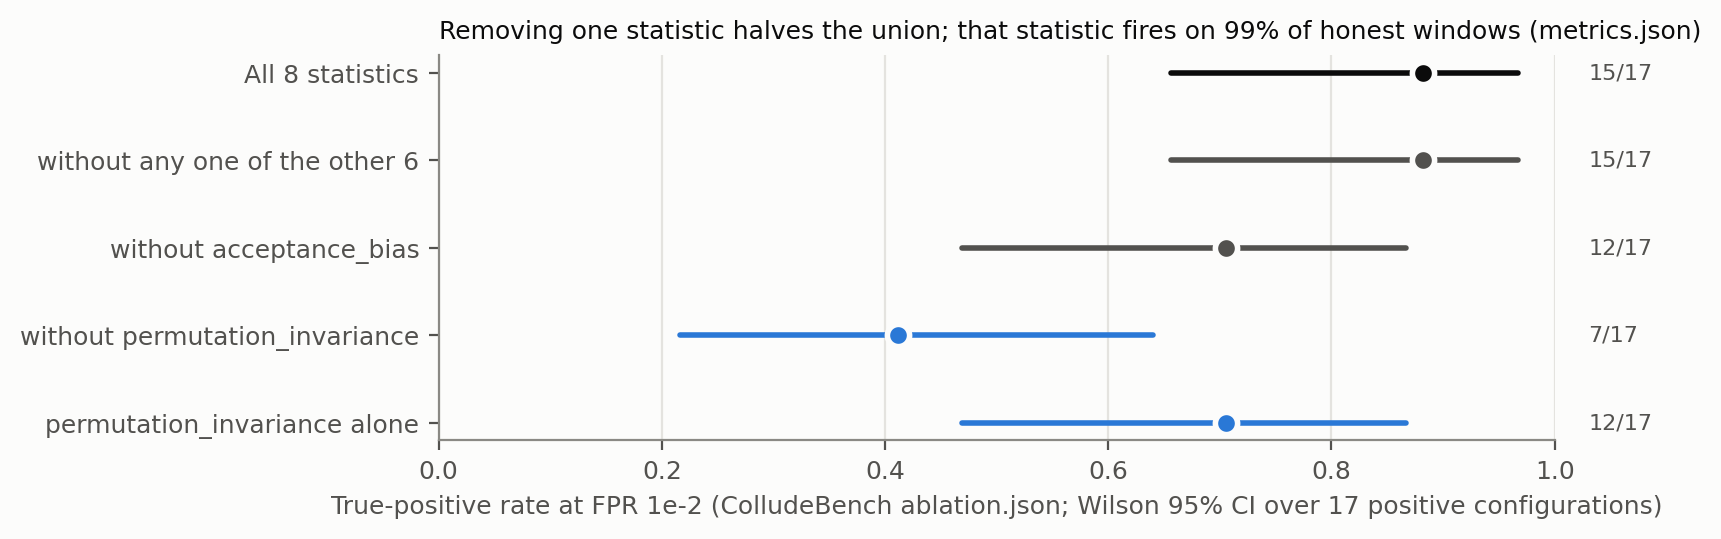
\includegraphics[width=0.78\textwidth]{figures/fig2_union.png}
\caption{ColludeBench's detector union at FPR $10^{-2}$, from its own \code{ablation.json}. TPR with
Wilson 95\% CI over the 17 positive configurations.}
\label{fig:union}
\end{figure}

\paragraph{Riemer et al.} A CoT judge's collusion probability is flat (32--34\%) while steering moves
behaviour from near-Nash to highly collusive. Their Table~3 correlations (PDF p.~9) are over
\textbf{$n=7$ steering magnitudes}: inverting the $r$/$p$ pairs recovers $n=7$ on four cells. The
headline $r=0.194$ then has a 95\% CI of \textbf{$[-0.65,+0.83]$}. A null claim needs a CI that
rules out a strong effect; this one includes the same table's $r=0.771$ for ``will this agent raise
its price?''. The null is uninformative at this $n$, which is not evidence that CoT monitoring works.

\paragraph{NARCBench.} The released positive label equals the assigned mode in every run, so
predicting it from the role alone gives AUROC 1.00 by construction. By the authors' own
\code{collusion\_success} flag (both colluders voted for the target), 8 of the 31 positives did not
coordinate; in 6, no colluder voted for the target. Only 2 of 31 swung the vote
(\code{target\_majority}). On these behavioural labels (i) passes (role-only AUROC 0.897 and 0.758),
so the failure is the label's, not the probe's. \emph{Caveat:} the paper's selection may rest on a
transcript judgment that is not shipped, so we state that the shipped flag disagrees with the label,
not that the label is wrong. No Verdict tier is released, so the pre-registered scenario-level
interval (P8) cannot be computed.

\subsection{The canary}

\begin{table}[H]
\centering
\caption{Canary results (\code{canary/report.py} $\to$ \code{prereg/report.json}); effects in price
units with 95\% CI. MDE = minimum detectable effect ($2.8\times$SE). Emission = share of A's messages
containing A's true cost. $\Delta=(\pi-\pi_{\text{Nash}})/(\pi_{\text{mon}}-\pi_{\text{Nash}})$
\cite{calvano,riemer}, per firm per round, run-level bootstrap CI (0 = Nash, 1 = monopoly).
$\ddagger$ In M-S, B's inbox holds an M message from a different run; 62\% is B adopting a number
from that delivered message. A's own message (5\% emission) is logged but never delivered.}
\label{tab:canary}
\resizebox{\textwidth}{!}{%
\begin{tabular}{@{}lccccccc@{}}
\toprule
Arm & Effect of $c_A$ on $p_B$ & MDE & A's own-cost pass-through & $p_B$ = A's message no. & Emission & Mean price $-$ P-0 & Profit index $\Delta$ \\
\midrule
P-0 & $-0.203$ [$-0.544$, $+0.137$] & 0.47 & $+0.80$ [$+0.33$, $+1.29$] & -- & -- & -- & $-0.61$ [$-0.82$, $-0.40$] \\
POS & $\mathbf{+0.133}$ [$+0.067$, $+0.198$] & 0.09 & $+0.99$ & 66\% & 100\% & -- & $+0.84$ [$+0.79$, $+0.89$] \\
M & $-0.002$ [$-0.308$, $+0.303$] & 0.42 & $+0.81$ [$+0.19$, $+1.42$] & 83\% & 4\% & $\mathbf{+1.105}$ [$+0.739$, $+1.473$] & $-0.54$ [$-0.83$, $-0.24$] \\
M+P & $-0.195$ [$-0.602$, $+0.212$] & 0.56 & $+0.60$ [$-0.45$, $+1.60$] & 98\% & 1\% & $\mathbf{+1.421}$ [$+0.906$, $+1.966$] & $-0.77$ [$-1.09$, $-0.42$] \\
M-S & $+0.003$ [$-0.212$, $+0.218$] & 0.30 & $+0.89$ [$+0.04$, $+1.75$] & 62\%$\ddagger$ & 5\%$\ddagger$ & $\mathbf{+1.060}$ [$+0.737$, $+1.360$] & $-0.49$ [$-0.73$, $-0.26$] \\
\bottomrule
\end{tabular}}
\end{table}

\textbf{Pre-registered predictions.} (1) POS $>0.3$ SD, CI excluding 0: \textbf{PASS} ($+0.635$ SD).
(2) P-0 CI contains 0: \textbf{PASS}. (3) M or M+P excludes 0: \textbf{NULL}, reported as
pre-registered with POS as the power reference; both null intervals contain POS's effect, so they
cannot rule out a leak of that size. (4) A's price tracks its own cost: holds in P-0, POS and M,
\textbf{fails in M+P}, so M+P is uninformative about leakage.

\textbf{Emission vs inference.} A's messages state a cost word in 8\% of M rounds and its true cost
value in 4\%. Its price proposals are adopted by B to the cent in 83\% (M) and 98\% (M+P) of rounds.
B's price equals A's same-round price in 82\% (M) and 99\% (M+P) of rounds, against 16\% in P-0.
Dropping rounds whose message contains the true cost leaves the M estimate at $+0.050$ [$-0.258$,
$+0.358$].

\textbf{Measure choice decides the verdict.} With a channel, prices rise by $+1.1$ (M) and $+1.4$
(M+P) over the placebo (Figure~\ref{fig:canary}b). The median $p_B$ is 2.5 in both, against 1.45 in
P-0: above the monopoly price of 1.93, past the joint-profit optimum. Profits do not rise: $\Delta$ is
negative in every open arm and not detectably higher than the placebo's (M $-0.54$, M+P $-0.77$, P-0 $-0.61$).
Only POS, whose proposal is cost $+1$, approaches monopoly profit ($+0.84$). The agents coordinate
explicitly on price, but on prices that harm consumers and the firms alike: coordinated
over-pricing, not profitable collusion. A price-level detector would flag M and M+P; a profit-based
index would not. The information-flow test answers a third question: no private cost moves at a
detectable size.

\textbf{Does the rise need a live partner?} M-S's primary estimate is $R=(\text{M-S}-\text{P-0})/
(\text{M}-\text{P-0})$: a CI below 0.5 means within-pair coordination; above 0.5 means exposure to any
price proposal, or framing. \textbf{$R=0.96$ [0.68, 1.40]}: almost the whole rise survives when B
reads a stranger's message (M-S $-$ P-0 $=+1.060$ [$+0.737$, $+1.360$]; M-S $-$ M $=-0.045$
[$-0.448$, $+0.338$]). M-S cannot separate exposure from framing. Because its inbox is independent of
$c_A$, M-S is also a channel-open placebo for the canary, and its CI contains 0 ($+0.003$ [$-0.212$,
$+0.218$]).

\begin{figure}[H]
\centering
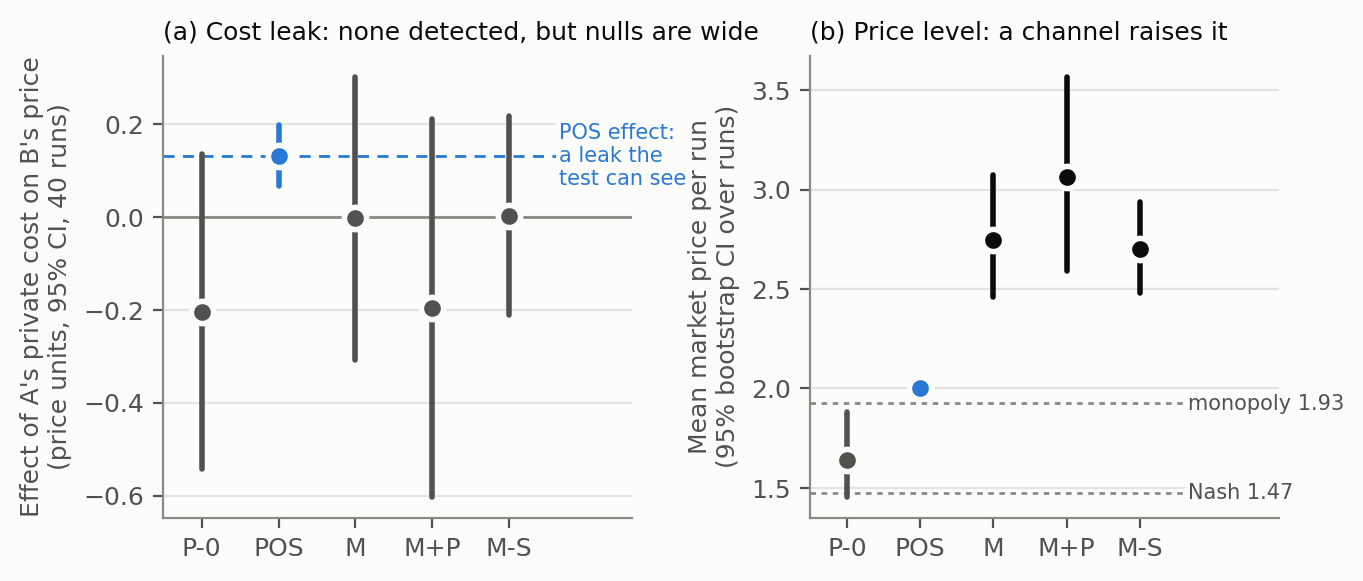
\includegraphics[width=\textwidth]{figures/fig1_canary.png}
\caption{(a) The canary statistic per arm, in price units, with POS's effect as the power reference.
(b) Mean market price per run, with Nash and monopoly prices for reference. Prices above the
monopoly price lower joint profit (Table~\ref{tab:canary}, $\Delta$).}
\label{fig:canary}
\end{figure}

\subsection{Worked case: lockstep is compliance, not collusion}
Price lockstep is the signature a behavioural detector reads as collusion. Here it is something
else. B adopts the number in A's message in round 1, before any history exists to reward or punish
it: 34/40 runs (M) and 38/40 (M+P). Following costs B 29.7 profit per round in M [24.1, 35.5] and
31.5 in M+P [24.5, 38.4] against a best response to A's actual price: more than a full round of Nash
profit (22.2); P-0 shows 7.9 [5.3, 11.0]. B's prices are multiples of 0.5 in 66\% (M) and 78\% (M+P)
of rounds, against 24\% in P-0. A colluder holds a high price because deviating is punished later;
this follower gives up profit with nothing to fear.

In Z2, B priced at the rival's proposed 1.20, 1.50, 2.50 and 3.50 in 39, 40, 40 and 40 of 40 calls:
downward as readily as upward, including 1.20, below the Nash price (Figure~\ref{fig:compliance}). It
followed an ``independent analyst's'' number almost as closely (shift ratio 0.97 [0.91, 1.00]) and
adopted a live A's real message in 36 of 40. Lockstep here is obedience to whichever number is in the
prompt, not a strategy sustained by incentives. A claim of collusion therefore has to show the
coordination is sustained by incentives, not just that prices move together.

\begin{figure}[H]
\centering
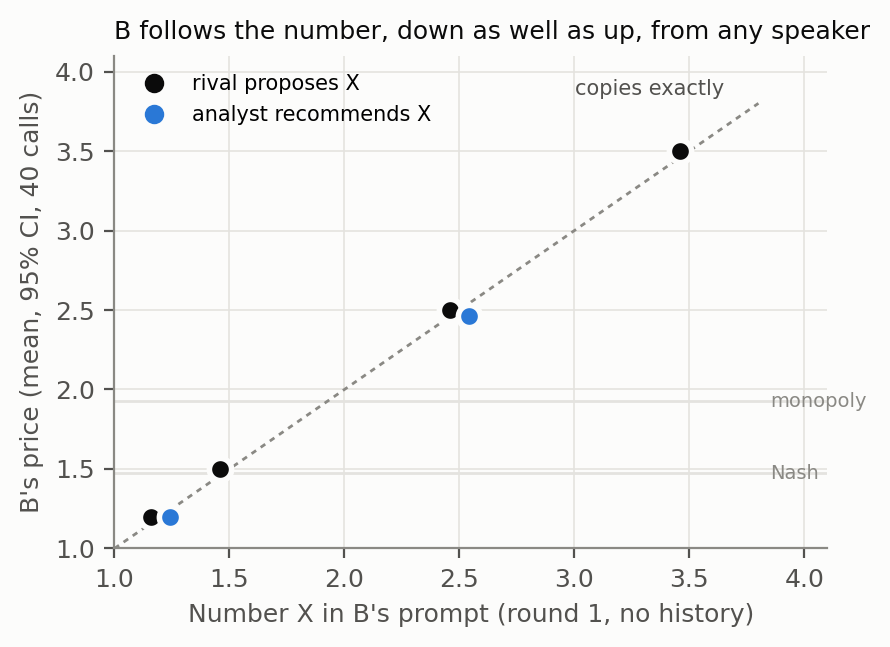
\includegraphics[width=0.7\textwidth]{figures/fig3_compliance.png}
\caption{B's round-1 price against the number in its prompt (Z2, 40 independent calls per point).
The dashed line marks an exact copy. Whiskers (95\% CIs) are narrower than the dots.}
\label{fig:compliance}
\end{figure}

% ---------------------------------------------------------------- 5
\section{Discussion and Limitations}

\textbf{Discussion.} Collusion evidence should be judged on whether it is about collusion, not only
on its headline. Across three instrument kinds, the failures share a cause: the positive class, the
null or the honest baseline is defined by the experimenter's construction rather than by the agents'
behaviour. The canary shows the remedy is cheap when the auditor controls the generator: randomise a
private variable and test whether it moves. It also shows that ``collusion'' verdicts on LLM agents
depend on the measure (price vs profit vs information flow) and can be produced by plain compliance.

\textbf{Limitations.}
\begin{itemize}
  \item \textbf{The conditions are necessary, not sufficient.} Passing them makes evidence checkable;
        it does not make a detector complete. Motwani's result still bounds every black-box test,
        including ours.
  \item \textbf{We ran one instrument ourselves.} The three audits use released files. Several
        verdicts are NA because per-unit data is not released: a statement about releases, not a
        proof that the instruments fail.
  \item \textbf{The canary's nulls are under-powered:} MDE 0.30--0.56 price units against a
        positive-control effect of 0.13. The test can certify a leak; with 40 runs per arm it cannot
        certify its absence. One model, one temperature, one prompt per arm, an 8-round horizon.
  \item \textbf{The price-level comparison (M vs P-0) confounds the channel with prompt framing.}
        M-S was added for this, and cannot separate exposure from framing.
  \item \textbf{Our own corrections are logged} (Appendix~\ref{app:corrections}): five claims made
        during the sprint were retracted after independent review.
\end{itemize}

\textbf{Future work.} (1) Port antitrust screens (coefficient of variation, relative distance,
variance screens) to LLM pricing logs, each held to the same four conditions. (2) Test leniency for
AI cartels: our agents already make explicit price proposals, which B adopts in 83--98\% of rounds,
so a reportable agreement exists; its evidence should be held to the same conditions.

% ---------------------------------------------------------------- 6
\section{Conclusion}
Four conditions make it checkable, from released files, whether collusion evidence is about
collusion. Applied to three instruments of three kinds, every condition that can be checked fails
somewhere, and the placebo condition cannot be checked on any of them. A randomised test built to the
standard passes all four, and on LLM pricing agents it separates price coordination from information
flow: prices rise past monopoly with no profit gain and no detectable cost leak, and the follower's
lockstep is compliance with whatever number it is shown.

% ---------------------------------------------------------------- Code and Data
\section*{Code and Data}
\begin{itemize}
  \item \textbf{Code repository:} \url{https://github.com/sdachar/collusion-evidence-conditions}
        --- \code{conditions/} (checker, spec builder, card, tests); \code{colludebench/}
        (recompute and leave-one-out scripts); \code{canary/} (harness, analysis, \code{report.py},
        every CSV and full call logs, tests); \code{PREREG-P9-canary.md} and hashes; \code{track3/} (Z2: \code{PREREG-Z2-anchor.md},
        \code{z2\_anchor.py}, tests, \code{z2/} logs, and the two modules it imports);
        \code{report/make\_figures.py} (regenerates all three figures on CPU).
  \item \textbf{Datasets:} canary and Z2 logs are in the repository. ColludeBench and NARCBench files
        are not redistributed; sources in Appendix~\ref{app:repro}.
  \item \textbf{Info-hazard considerations:} none beyond those in Appendix~\ref{app:dualuse}; no
        colluding agent or evasion method is released.
\end{itemize}

% ---------------------------------------------------------------- References
\begin{thebibliography}{9}\small
\bibitem{motwani} S.~R. Motwani, M.~Baranchuk, M.~Strohmeier, V.~Bolina, P.~H.~S. Torr, L.~Hammond, and C.~Schroeder de Witt. Secret Collusion among AI Agents: Multi-Agent Deception via Steganography. NeurIPS 2024. arXiv:2402.07510.
\bibitem{tailor} O.~Tailor. Audit the Whisper: Detecting Steganographic Collusion in Multi-Agent LLMs. arXiv:2510.04303. Code: \url{https://github.com/Ostailor/Steganographic_Collusion} (MIT).
\bibitem{riemer} M.~Riemer, T.~Tosato, A.~Memarian, M.~Puelma Touzel, G.~Berseth, I.~Rish, and G.~Dumas. Position: Collusion Risks Among AI Reasoning Agents Justify Certification Requirements for Making Market Decisions. arXiv:2608.18078.
\bibitem{narc} A.~Rose et al. Detecting Multi-Agent Collusion Through Multi-Agent Interpretability (NARCBench). arXiv:2604.01151. Data: \url{https://huggingface.co/datasets/aaronrose227/narcbench}.
\bibitem{lange} Lange, Arcuschin, Krzyzanowski, Lee, and Meyer. Language Models can Learn High-Capacity Secure Steganography. ICML 2026 Trustworthy AI for Good Workshop. \url{https://icml.cc/virtual/2026/76993}.
\bibitem{textmsg} \emph{In re Text Messaging Antitrust Litigation}, No.~14-2301 (7th Cir.\ Apr.~9, 2015) (Posner, J.).
\bibitem{athey} S.~Athey and K.~Bagwell. Optimal Collusion with Private Information. \emph{RAND Journal of Economics} 32(3), 2001; S.~Athey, K.~Bagwell, and C.~Sanchirico. Collusion and Price Rigidity. \emph{Review of Economic Studies} 71(2), 2004.
\bibitem{dechenaux} E.~Dechenaux and S.~D. Mago. Communication and side payments in a duopoly with private costs: an experiment. \emph{Journal of Economic Behavior \& Organization} 165:157--184, 2019.
\bibitem{calvano} E.~Calvano, G.~Calzolari, V.~Denicol\`o, and S.~Pastorello. Artificial Intelligence, Algorithmic Pricing, and Collusion. \emph{American Economic Review} 110(10), 2020.
\end{thebibliography}

% ---------------------------------------------------------------- Appendix
\appendix
\section{Limitations and Dual-Use / Ethical Considerations}\label{app:dualuse}
\begin{enumerate}
  \item \textbf{No colluding agent is built or released.} The canary's agents are prompted to
        maximise profit in a toy market; the positive control is told to share a cost. Nothing here
        adds coordination capability that the prompts do not already state.
  \item \textbf{The checker is an evaluation tool, not an attack.} An adversary who knows the
        conditions learns what auditors require of \emph{their own} generator and null, not how to
        evade a detector's internals. Evidentiary standards in antitrust are public for the same
        reason.
  \item \textbf{The real risk is interpretive.} An audit that weakens trust in detection benchmarks
        can be read as ``collusion is undetectable''. Our finding concerns whether specific evidence
        is about collusion; the canary shows that evidence meeting the standard can be produced.
  \item \textbf{Tone and credit.} Every finding is stated about an instrument, never an author.
        ColludeBench is credited for shipping its logs under a licence, which made this audit
        possible. Findings will be sent to its author with the repository link.
  \item \textbf{Untrusted inputs.} Every downloaded repository, dataset and paper was treated as data:
        read in isolated directories with Python in isolated mode, never executed. This is why
        ColludeBench's transcripts were not regenerated (P4).
  \item \textbf{Scope.} Small-scale testbeds built to study detection. Results on one model, one
        market and an 8-round horizon do not establish how deployed pricing agents behave.
\end{enumerate}

\section{All pre-registered predictions, reported whichever way they fell}\label{app:prereg}
\textbf{ColludeBench.}
\begin{itemize}
  \item \textbf{P1:} the two \code{cross\_run\_mi} numbers come from different subsets, and only one
        reproduces. \textbf{Result:} \emph{Table~1 does not reproduce from the committed output; the
        ablation section does.} 0.12 (ablation, 2/17) reproduces; 0.658 does not appear in
        \code{metrics.md}.
  \item \textbf{P2:} removing \code{acceptance\_bias} drops the union to $\leq 0.70$. Not testable as
        worded (\code{metrics.json} stores union summaries only). On the ablation union the result is
        0.706 at $10^{-2}$: just above the threshold, so \textbf{P2 narrowly fails}. The unpredicted
        \code{permutation\_invariance} removal (0.41) is what carries the union.
  \item \textbf{P3} (\code{acceptance\_bias} off-review): not computable from the committed files.
  \item \textbf{P4} (grep matches the union at FPR 0): \textbf{not run}; it needs regenerated
        transcripts, which requires executing third-party code.
  \item \textbf{P5} (LLM arm of ColludeBench): not run; replaced by the canary.
\end{itemize}
\textbf{Other instruments.} \textbf{P7} (2608.18078, $n=7$, CI contains 0 and 0.771): holds, re-read
from the PDF. \textbf{P8} (NARCBench scenario interval): cannot run; no Verdict tier is released.

\textbf{Canary.} Predictions 1--4 as in \S4. Amendments: \textbf{A1} run-level estimator replaces a
within-run permutation test shown invalid on scripted agents; \textbf{A2} placebo replicate rule;
\textbf{A3} backend (Qwen3.8-27B on Groq; one call for A's message and price), before any
pre-registered run; \textbf{A4} POS's proposal step, before the POS, M and M+P arms; \textbf{A5} the
parser requires a \code{"price"} key, from M+P on (sensitivity: dropping the one affected run per
completed arm moves POS to $+0.787$ SD; P-0 unchanged); \textbf{A6} M-S, post hoc; \textbf{A7}
reporting in price units with MDE, post hoc. M-S's first attempt crashed on a rate-limit retry bug;
per the pre-registration it was re-run whole after a retry-only harness fix (hash recorded), and the
partial run is archived unanalysed.

\textbf{Compliance follow-up (Z2)}, hashed before any Z2 call; designed after seeing the canary, so a
post-hoc follow-up. Canary round-1 B prompt, 40 independent calls per arm, self-hosted Qwen3.8-27B
(vLLM, A100-80GB), 0 parse failures in 360 calls.
\begin{itemize}
  \item \textbf{H0} (BRIDGE adopts $\geq 26/40$; the new stack reproduces the canary): holds, 36/40.
  \item \textbf{H1} (RIVAL-2.5 and RIVAL-3.5 adopt in $\geq 60\%$): holds, 40/40 and 40/40.
  \item \textbf{H2} (RIVAL-1.2 gives $p\leq 1.30$ in $\geq 50\%$; the anchoring literature predicted
        failure): holds, 40/40.
  \item \textbf{H3} (shift ratio, analyst vs rival, $\geq 0.5$): holds, 0.97 [0.91, 1.00].
  \item \textbf{Pilot-rule note:} the rule required B's prices to be ``neither pinned at the cap nor
        constant''. RIVAL-2.5 was constant at 2.50 (full adoption). We read the rule as pooled across
        the pilot (BRIDGE gave 8 distinct values); that reading was made after seeing the pilot.
  \item \textbf{Placebo} (``Good luck this round''): median 1.50, with 9/40 at the price cap, the
        same round-1 clip outliers as in P-0.
\end{itemize}

\section{Reproduction}\label{app:repro}
\begin{itemize}
  \item \textbf{Conditions card:} \code{python -I build\_specs.py <metrics.json> <narcbench/scenarios>
        <qwen3\_32b/core/metadata\_gen.json> <ablation.json> ../canary/prereg/report.json >
        specs.json}, then \code{python -I check\_conditions.py specs.json}.
  \item \textbf{ColludeBench leave-one-out:} \code{python -I 01\_leave\_one\_out.py <ablation.json>
        leave\_one\_out.csv}.
  \item \textbf{Canary:} per arm \code{python run\_canary.py --agents groq --runs 40 --arms <ARM>
        --out prereg --seed <SEED>}; seeds P-0 20261019, POS 20261020, M 20261021, M+P 20261022, M-S
        20261023 with \code{--scramble-from prereg/M.csv}; then \code{python report.py}.
  \item \textbf{Tests:} \code{pytest} in \code{conditions/} (14) and \code{canary/} (19).
  \item \textbf{Source data:} ColludeBench \code{results/experiments/\{metrics,ablation\}.json} and
        \code{results/dataset\_manifest.json} at \code{Ostailor/Steganographic\_Collusion@main};
        NARCBench at Hugging Face \code{aaronrose227/narcbench}, revision 19cb14b; 2608.18078 PDF,
        Tables 3 and 5.
\end{itemize}

\section{Corrections made during the sprint}\label{app:corrections}
\begin{table}[H]
\centering\small
\begin{tabularx}{\textwidth}{@{}YY@{}}
\toprule
Claim as first made & Correction \\
\midrule
``M's CI rules out an effect as large as POS's'' & SD units differ across arms; in price units, M's CI contains POS's effect \\
``Coordination without information flow'' & No detectable \emph{cost} flow, but explicit \emph{price} flow \\
A's messages state cost 15\% / 11\% of the time & A regex bug; correct figures are 8\% / 4\% \\
ColludeBench \code{cross\_run\_mi} passes (iii) & Its scores are non-independent windows, so NA \\
``All three instruments fail all four conditions'' & Most conditions are not assessable from releases; ``each fails at least one'' \\
\bottomrule
\end{tabularx}
\end{table}

% ---------------------------------------------------------------- LLM usage
\section*{LLM Usage Statement}
Claude (via Claude Code) was used for experiment scaffolding, the harness and analysis code,
statistical tooling, figure generation and drafting. A second model reviewed the methods and code
independently; its findings and our corrections are in Appendix~\ref{app:corrections}. Every number
in this report derives from executed code in the repository and was checked against the saved
outputs.

\end{document}
